\chapter{Perancangan}

\section{Perancangan Aplikasi Mesin Navigasi KIRI}

Seperti telah dibahas pada bab analisis, ada beberapa penambahan kelas pada mesin navigasi KIRI. Adapun kelas utama yang ditambahkan adalah kelas \texttt{DataPuller} yang bertanggung jawab untuk menarik data dari Peta Angkutan Umum. Kelas ini memiliki beberapa \textit{method} antara lain:

\begin{itemize}
	\item \textbf{public void (File sqlPropertiesFile, PrintStream output)} \\
		Berfungsi untuk memeriksa seluruh trayek di basis data. Untuk trayek yang memenuhi syarat (terintegrasi dengan Peta Angkutan Umum dan terdapat data yang lebih baru di Peta Angkutan Umum), melakukan penarikan. \\
		\textbf{Parameter:}
		\begin{itemize}
			\item \textbf{sqlPropertiesFile} menunjukkan berkas yang menyimpan konfigurasi dari basis data yang akan digunakan.
			\item \textbf{output} tempat di mana hasil dari penarikan akan ditulis (pada umumnya akan ditulis ke berkas tracks.conf).
		\end{itemize}
		\textbf{Kembalian:} tidak ada.
	\item \textbf{private static LngLatAlt[] lineStringToLngLatArray(String wktText)} \\
		\textit{Method} bantuan untuk mengubah teks dari format \textit{Well-known text} \cite{Herring:2011} menjadi \textit{array} \textit{latitude} dan \textit{longitude}. Hal ini diperlukan karena MySQL mengembalikan data rute dalam format \textit{Well-known text} tersebut, sedangkan pemrosesan dalam bahasa Java lebih mudah jika datanya memiliki struktur. \\
		\textbf{Parameter:}
		\begin{itemize}
			\item \textbf{wktText} Teks yang berisi data rute dalam format \textit{Well-known text}
		\end{itemize}
		\textbf{Kembalian:} rute dalam \textit{array} \textit{latitude} dan \textit{longitude}
	\item \textbf{private static double computeDistance(LngLatAlt p1, LngLatAlt p2)} \\
		\textit{Method} bantuan untuk menghitung jarak dari dua buah titik dalam format \textit{latitude} dan \textit{longitude}. Perhitungannya menggunakan metode \textit{haversine}\footnote{http://www.movable-type.co.uk/scripts/latlong.html}.
		\textbf{Parameter:}
		\begin{itemize}
			\item \textbf{p1} titik pertama
			\item \textbf{p2} titik kedua
		\end{itemize}
		\textbf{Kembalian:} jarak kedua titik tersebut dalam kilometer
	\item \textbf{private RouteResult formatTrack(String trackTypeId, String trackId,
			LngLatAlt[] geodata, boolean isPathLoop, String penalty,
			String transferNodesStr, int lastUpdate))} \\
		Mengkonversikan sebuah data trayek dalam format yang digunakan pada berkas tracks.conf. \\
		\textbf{Parameter:}
		\begin{itemize}
			\item \textbf{trackTypeId} kode tipe trayek
			\item \textbf{trackId} kode trayek angkot
			\item \textbf{geodata} titik kedua
			\item \textbf{isPathLoop} titik kedua
			\item \textbf{penalty} titik kedua
			\item \textbf{transferNodeStr} titik kedua
			\item \textbf{lastUpdate} titik kedua
		\end{itemize}
		\textbf{Kembalian:} informasi rute dalam format berkas tracks.conf
	\item \textbf{private RouteResult formatTrackFromAngkotWebId(String angkotId, String trackTypeId, String trackId)} \\
		Mengkonversikan data dari situs Peta Angkutan Umum menjadi format yang digunakan pada berkas tracks.conf.
		\textbf{Parameter:}
		\begin{itemize}
			\item \textbf{angkotId} kode angkot pada Peta Angkutan Umum
			\item \textbf{trackTypeId} kode tipe trayek
			\item \textbf{trackId} kode trayek angkot
		\end{itemize}
		\textbf{Kembalian:} informasi rute dalam format berkas tracks.conf
\end{itemize}

Selain itu, peneliti juga membuat kelas lain \texttt{RouteResult} yang merupakan \textit{inner class} dari \texttt{DataPuller}, untuk menampung hasil dari pembuatan rute serta pembacaan rute dari Peta Angkutan Umum. Kelas ini memiliki beberapa atribut antara lain:

\begin{itemize}
	\item int \textbf{lastUpdate} \\
		Menyimpan tanggal terakhir rute ini diperbaharui di Peta Angkutan Umum dalam format UNIX time.
	\item String \textbf{trackInConfFormat} \\
		Menyimpan representasi rute ini dalam format berkas tracks.conf.
	\item String \textbf{trackInMySQLFormat} \\
		Menyimpan representasi rute ini dalam format query MySQL.
\end{itemize}

Kelas \texttt{RouteResult} tidak memiliki method kecuali konstruktor dan \textit{getter}.

Terakhir, ditambahkan pula kelas \texttt{DataPullerException} untuk mencatat segala eksepsi pada saat menarik data dari Peta Angkutan Umum.

Detail seluruh kelas yang ditambahkan dapat dilihat pada kelas diagram pada gambar \ref{fig:4_diagram_kelas}.

\begin{figure}
	\centering
	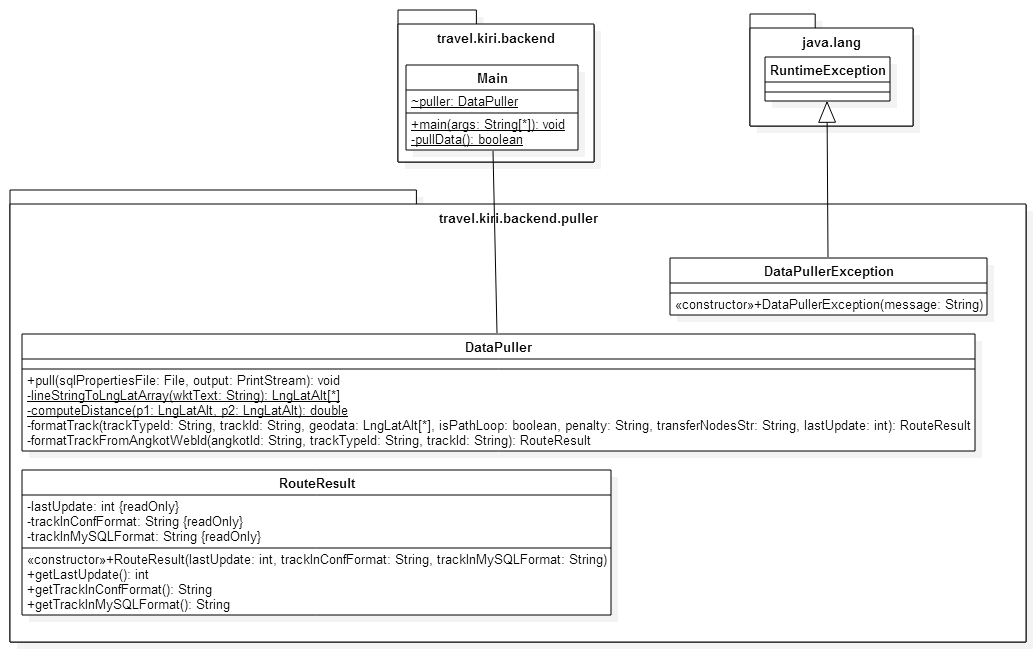
\includegraphics[scale=0.45]{Gambar/4_diagram_kelas}
	\caption{Diagram Kelas (Tahap Desain)} 
	\label{fig:4_diagram_kelas}
\end{figure}

\section{Perancangan Protokol}

Protokol untuk melakukan sinkronisasi dibuat di atas protokol \textit{Transportation List} dan \textit{Transportation Detail} milik situs Peta Angkutan Umum. Di awal sinkronisasi, mesin navigasi KIRI mencatat trayek apa saja yang harus disinkronkan dengan Peta Angkutan Umum. Kemudian, mesin navigasi KIRI akan mengirimkan permintaan \textit{Transportartion List} dengan menyertakan parameter id/kode angkot Peta Angkutan Umum, yang dipisahkan dengan \textit{pipe} ("|"). Tambahan parameter ini merupakan hasil dari optimasi protokol yang sudah ada, sehingga jawaban yang dikirimkan hanya mencakup angkot yang diperlukan oleh KIRI saja.

Contohnya, permintaan \textit{Transportation List} yang meminta status dari angkot dengan kode 1 dan 2 saja menggunakan perintah \texttt{GET /route/transportation-list.json?id=1|2}. Hasil dari permintaan tersebut akan menghasilkan kembalian kurang lebih seperti berikut:

\begin{lstlisting}
{
   "transportations":[
      {
         "city":"Jakarta",
         "id":1,
         "updated":"1381097188",
         "number":"M17",
         "province":"ID-JK",
         "company":"Mikrolet",
         "created":"1376493332",
         "destination":"Pasar Lenteng Agung",
         "origin":"Pasar Minggu",
         "hasRoute":true
      },
      {
         "city":"Jakarta",
         "id":2,
         "updated":"1379737743",
         "number":"S616",
         "province":"ID-JK",
         "company":"Kopaja",
         "created":"1376494541",
         "destination":"Cipedak",
         "origin":"Blok M",
         "hasRoute":true
      }
   ],
   "status":"ok",
   "provinces":[
      [
         "ID-AC",
         "Aceh"
      ],
      ...
    ]
}
\end{lstlisting}

Dari kembalian di atas, mesin navigasi KIRI dapat mengetahui kapan rute di Peta Angkutan Umum terakhir diperbaharui, untuk trayek-trayek yang diminta. Untuk setiap rute yang telah berubah, KIRI mengirimkan lagi perintah berikutnya, yaitu \textit{Transportation Detail}, yang memberikan rute penuh untuk trayek yang diminta. Sebagai contoh, jika rute dengan kode 1 ditemukan telah berubah, maka akan dikirimkan perintah \textit{Transportation Detail} \texttt{GET /route/transportation/1.json}. Dari situ, rute lengkap akan disimpan pada berkas \texttt{tracks.conf}.

\section{Perancangan Antarmuka}

\subsection{Antarmuka Mesin Navigasi KIRI}

Mesin navigasi KIRI adalah program yang dijalankan sebagai server, sehingga hanya memiliki antarmuka minimal berbasis teks yang menampilkan aksi-aksi yang dilakukan oleh server. Setelah ditambahkan fitur menarik data dari Peta Angkutan Umum, maka akan ada tambahan penampilan aksi menarik rute seperti contoh berikut (tambahan ada pada baris 1-8):

\begin{lstlisting}
May 20, 2015 1:56:02 PM travel.kiri.backend.puller.DataPuller pull
INFO: Fetching https://angkot.web.id/route/transportation-list.json?id=157|247|636...
May 20, 2015 1:56:11 PM travel.kiri.backend.puller.DataPuller formatTrackFromAngkotWebId
INFO: Fetching bdo_angkot.cicaheumciroyom from https://angkot.web.id/route/transportation/157.json...
May 20, 2015 1:56:17 PM travel.kiri.backend.puller.DataPuller formatTrackFromAngkotWebId
INFO: Fetching bdo_angkot.cicaheumledeng from https://angkot.web.id/route/transportation/247.json...
May 20, 2015 1:56:19 PM travel.kiri.backend.puller.DataPuller formatTrackFromAngkotWebId
INFO: Fetching bdo_angkot.ciroyomantapani from https://angkot.web.id/route/transportation/636.json...
May 20, 2015 1:56:37 PM travel.kiri.backend.Worker <init>
INFO: Configuration were read successfully
May 20, 2015 1:56:41 PM travel.kiri.backend.Worker <init>
INFO: Tracks were read successfully
May 20, 2015 1:57:04 PM travel.kiri.backend.Worker <init>
INFO: Tracks were linked successfully
2015-05-20 13:57:07.356:INFO::main: Logging initialized @65987ms
2015-05-20 13:57:10.173:INFO:oejs.Server:main: jetty-9.2.3.v20140905
2015-05-20 13:57:11.483:INFO:oejs.ServerConnector:main: Started ServerConnector@2996771e{HTTP/1.1}{0.0.0.0:8000}
2015-05-20 13:57:11.485:INFO:oejs.Server:main: Started @70398ms"
\end{lstlisting}


\subsection{Antarmuka Situs Web KIRI}

Pada situs web KIRI, jika ditemukan rute yang dihasilkan terintegrasi dengan Peta Angkutan Umum, maka situs akan menambahkan sebuah tombol kecil berbentuk pensil, yang jika diklik akan membawa pengguna ke situs Peta Angkutan Umum untuk memodifikasi rute terkait. Tampilan tombol tersebut dapat dilihat di \ref{fig:4_tombolubah}.

\begin{figure}
	\centering
	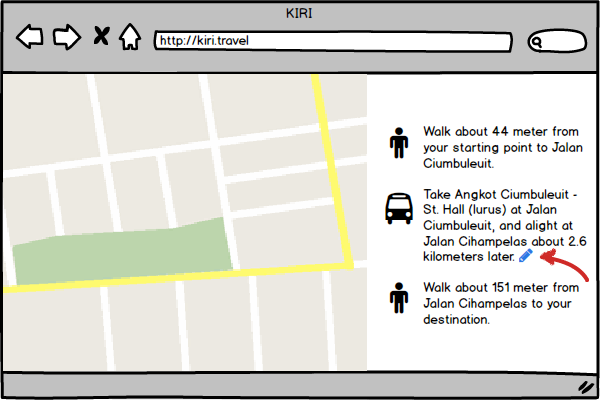
\includegraphics[scale=0.5]{Gambar/4_tombolubah}
	\caption{Tombol ubah di situs web KIRI} 
	\label{fig:4_tombolubah}
\end{figure}